%% abtex2-modelo-trabalho-academico, v-1.9.7 laurocesar
%% Copyright 2012-2018 by abnTeX2 group at http://www.abntex.net.br/ 
%%
%% This work may be distributed and/or modified under the
%% conditions of the LaTeX Project Public License, either version 1.3
%% of this license or (at your option) any later version.
%% The latest version of this license is in
%%   http://www.latex-project.org/lppl.txt
%% and version 1.3 or later is part of all distributions of LaTeX
%% version 2005/12/01 or later.
%%
%% This work has the LPPL maintenance status `maintained'.
%% 
%% The Current Maintainer of this work is the abnTeX2 team, led
%% by Lauro César Araujo. Further information are available on 
%% http://www.abntex.net.br/
%%
%% This work consists of the files abntex2-modelo-trabalho-academico.tex,
%% abntex2-modelo-include-comandos and abntex2-modelo-references.bib
%%

% ------------------------------------------------------------------------
% ------------------------------------------------------------------------
% abnTeX2: Modelo de Trabalho Academico (tese de doutorado, dissertacao de
% mestrado e trabalhos monograficos em geral) em conformidade com 
% ABNT NBR 14724:2011: Informacao e documentacao - Trabalhos academicos -
% Apresentacao
% ------------------------------------------------------------------------
% ------------------------------------------------------------------------

\documentclass[
	% -- opções da classe memoir --
	12pt,				% tamanho da fonte
	openright,			% capítulos começam em pág ímpar (insere página vazia caso preciso)
	twoside,			% para impressão em recto e verso. Oposto a oneside
	a4paper,			% tamanho do papel. 
	% -- opções da classe abntex2 --
	%chapter=TITLE,		% títulos de capítulos convertidos em letras maiúsculas
	%section=TITLE,		% títulos de seções convertidos em letras maiúsculas
	%subsection=TITLE,	% títulos de subseções convertidos em letras maiúsculas
	%subsubsection=TITLE,% títulos de subsubseções convertidos em letras maiúsculas
	% -- opções do pacote babel --
	english,			% idioma adicional para hifenização
	brazil				% o último idioma é o principal do documento
	]{abntex2}

% ---
% Pacotes básicos 
% ---
\usepackage{lmodern}			% Usa a fonte Latin Modern			
\usepackage[T1]{fontenc}		% Selecao de codigos de fonte.
\usepackage[utf8]{inputenc}		% Codificacao do documento (conversão automática dos acentos)
\usepackage{indentfirst}		% Indenta o primeiro parágrafo de cada seção.
\usepackage{color}				% Controle das cores
\usepackage{graphicx}			% Inclusão de gráficos
\usepackage{microtype} 			% para melhorias de justificação
% ---
		
% ---
% Pacotes adicionais, usados apenas no âmbito do Modelo Canônico do abnteX2
% ---
\usepackage{lipsum}				% para geração de dummy text
% ---

% ---
% Pacotes de citações
% ---
\usepackage[brazilian,hyperpageref]{backref}	 % Paginas com as citações na bibl
\usepackage[alf]{abntex2cite}	% Citações padrão ABNT

% --- 
% CONFIGURAÇÕES DE PACOTES
% --- 

% ---
% Configurações do pacote backref
% Usado sem a opção hyperpageref de backref
\renewcommand{\backrefpagesname}{Citado na(s) página(s):~}
% Texto padrão antes do número das páginas
\renewcommand{\backref}{}
% Define os textos da citação
\renewcommand*{\backrefalt}[4]{
	\ifcase #1 %
		Nenhuma citação no texto.%
	\or
		Citado na página #2.%
	\else
		Citado #1 vezes nas páginas #2.%
	\fi}%
% ---

% ---
% Informações de dados para CAPA e FOLHA DE ROSTO
% ---
\titulo{PIM VI \\ Projeto Integrado Multidiciplinar VI}
\autor{Pedro José Laurenti de Matos (RA:0621134)\\
}
\local{Anápolis, GO - Brasil}
\data{Maio de 2023}
\orientador{Davi Lazer Grave Teixeira
de Andrade}
\instituicao{
  Universidade Paulista -- UNIP
  \par
  Curso de Análise e Desenvolvimento de Sistemas
  \par
  Programa de Pós-Graduação}
\tipotrabalho{Trabalho Científico}
% O preambulo deve conter o tipo do trabalho, o objetivo, 
% o nome da instituição e a área de concentração 
\preambulo{Trabalho científico produzido para colocar em prática as habilidades adquiridas no segundo período do curso de Análise e Desenvolvimento de Sistemas.}
% ---


% ---
% Configurações de aparência do PDF final

% alterando o aspecto da cor azul
\definecolor{blue}{RGB}{41,5,195}

% informações do PDF
\makeatletter
\hypersetup{
     	%pagebackref=true,
		pdftitle={\@title}, 
		pdfauthor={\@author},
    	pdfsubject={\imprimirpreambulo},
	    pdfcreator={Pedro Laurenti},
		pdfkeywords={Desenvolvimento de Software}{Análise e Desenvolvimento de Sistemas}{ABNT LaTex}{Projeto Integrado Multidiciplinar V}{trabalho acadêmico}, 
		colorlinks=true,       		% false: boxed links; true: colored links
    	linkcolor=blue,          	% color of internal links
    	citecolor=blue,        		% color of links to bibliography
    	filecolor=magenta,      		% color of file links
		urlcolor=blue,
		bookmarksdepth=4
}
\makeatother
% --- 

% ---
% Posiciona figuras e tabelas no topo da página quando adicionadas sozinhas
% em um página em branco. Ver https://github.com/abntex/abntex2/issues/170
\makeatletter
\setlength{\@fptop}{5pt} % Set distance from top of page to first float
\makeatother
% ---

% ---
% Possibilita criação de Quadros e Lista de quadros.
% Ver https://github.com/abntex/abntex2/issues/176
%
\newcommand{\quadroname}{Quadro}
\newcommand{\listofquadrosname}{Lista de quadros}

\newfloat[chapter]{quadro}{loq}{\quadroname}
\newlistof{listofquadros}{loq}{\listofquadrosname}
\newlistentry{quadro}{loq}{0}

% configurações para atender às regras da ABNT
\setfloatadjustment{quadro}{\centering}
\counterwithout{quadro}{chapter}
\renewcommand{\cftquadroname}{\quadroname\space} 
\renewcommand*{\cftquadroaftersnum}{\hfill--\hfill}

\setfloatlocations{quadro}{hbtp} % Ver https://github.com/abntex/abntex2/issues/176
% ---

% --- 
% Espaçamentos entre linhas e parágrafos 
% --- 

% O tamanho do parágrafo é dado por:
\setlength{\parindent}{1.3cm}

% Controle do espaçamento entre um parágrafo e outro:
\setlength{\parskip}{0.2cm}  % tente também \onelineskip

% ---
% compila o indice
% ---
\makeindex
% ---

% ----
% Início do documento
% ----
\begin{document}

% Seleciona o idioma do documento (conforme pacotes do babel)
%\selectlanguage{english}
\selectlanguage{brazil}

% Retira espaço extra obsoleto entre as frases.
\frenchspacing 

% ----------------------------------------------------------
% ELEMENTOS PRÉ-TEXTUAIS
% ----------------------------------------------------------
% \pretextual

% ---
% Capa
% ---
\imprimircapa
% ---

% ---
% Folha de rosto
% (o * indica que haverá a ficha bibliográfica)
% ---
\imprimirfolhaderosto*
% ---

% ---
% Inserir a ficha bibliografica
% ---

% Isto é um exemplo de Ficha Catalográfica, ou ``Dados internacionais de
% catalogação-na-publicação''. Você pode utilizar este modelo como referência. 
% Porém, provavelmente a biblioteca da sua universidade lhe fornecerá um PDF
% com a ficha catalográfica definitiva após a defesa do trabalho. Quando estiver
% com o documento, salve-o como PDF no diretório do seu projeto e substitua todo
% o conteúdo de implementação deste arquivo pelo comando abaixo:
%
% \begin{fichacatalografica}
%     \includepdf{fig_ficha_catalografica.pdf}
% \end{fichacatalografica}

\begin{fichacatalografica}
	\sffamily
	\vspace*{\fill}					% Posição vertical
	\begin{center}					% Minipage Centralizado
	\fbox{\begin{minipage}[c][8cm]{13.5cm}		% Largura
	\small
	\imprimirautor
	%Sobrenome, Nome do autor
	
	\hspace{0.5cm} PIM V Projeto Integrado Multidiciplinar V --
	\imprimirlocal, \imprimirdata \ --
	
	\hspace{0.5cm} \thelastpage p.\\
	
	\hspace{0.5cm} \imprimirorientadorRotulo~\imprimirorientador\\
	
	\hspace{0.5cm}
	\parbox[t]{\textwidth}{\imprimirtipotrabalho~--~\imprimirinstituicao,
	\imprimirdata.}\\
	
	\hspace{5cm}
		1. Sistemas. \ \
		2. Desenvolvimento de Software. \ \
		3. Análise e Desenvolvimento de Sistemas. \ \
		4. ABNT LaTex \ \
		5. Universidade UNIP. \ \
		6. Levantamento de requisitos. \ \
		7. Projeto Integrado Multidiciplinar V. \ \		
	\end{minipage}}
	\end{center}
\end{fichacatalografica}

% ---
% Inserir folha de aprovação
% ---

% Isto é um exemplo de Folha de aprovação, elemento obrigatório da NBR
% 14724/2011 (seção 4.2.1.3). Você pode utilizar este modelo até a aprovação
% do trabalho. Após isso, substitua todo o conteúdo deste arquivo por uma
% imagem da página assinada pela banca com o comando abaixo:
%
% \begin{folhadeaprovacao}
% \includepdf{folhadeaprovacao_final.pdf}
% \end{folhadeaprovacao}
%
\begin{folhadeaprovacao}

\begin{center}
	{\ABNTEXchapterfont\large\imprimirautor}

	\vspace*{\fill}\vspace*{\fill}
	\begin{center}
	\ABNTEXchapterfont\bfseries\Large\imprimirtitulo
	\end{center}
	\vspace*{\fill}
	
	\hspace{.45\textwidth}
	\begin{minipage}{.5\textwidth}
		\imprimirpreambulo
	\end{minipage}%
	\vspace*{\fill}
\end{center}
		
Trabalho aprovado. \imprimirlocal, 22 de maio de 2023:

\assinatura{\textbf{\imprimirorientador} \\ Orientador} 
\assinatura{\textbf{Professor} \\ Convidado}
%\assinatura{\textbf{Professor} \\ Convidado 2}
%\assinatura{\textbf{Professor} \\ Convidado 3}
%\assinatura{\textbf{Professor} \\ Convidado 4}
	
\begin{center}
	\vspace*{0.5cm}
	{\large\imprimirlocal}
	\par
	{\large\imprimirdata}
	\vspace*{1cm}
\end{center}

\end{folhadeaprovacao}
% ---


% ---
% Dedicatória
% ---
\begin{dedicatoria}
	\vspace*{\fill}
	\centering
	\noindent
	\textit{Este projeto é dedicado a todos os desenvolvedores que já falharam várias vezes, mas nunca desistiram de suas paixões e ideias.}
 
	//
 
	\begin{quote}
	 \textit{``Herdei de meus ancestrais a tarefa de melhorar este mundo. E, para que possa entregá-lo a meus descendentes em melhor estado do que recebi, devo trabalhar, tanto quanto eles trabalharam ou ainda mais.'' - Bernard Shaw.}
	\end{quote}
 
	\vspace*{\fill}
 
 \end{dedicatoria}
 % ---
 

% ---
% Agradecimentos
% ---
\begin{agradecimentos}
	Os agradecimentos principais são direcionados à todos aqueles que contribuíram para que a produção deste trabalho acadêmico.
	
	Agradecimentos especiais são direcionados aos desenvolvedores do \abnTeX.
	
	\end{agradecimentos}
	% ---

% ---
% Epígrafe
% ---
\begin{epigrafe}
	\vspace*{\fill}
	\begin{flushright}
		\textit{``A máquina moderna é um instrumento de poder sem precedentes;\\ e sua falha é que não há precedentes que possam nos ensinar como lidar com isso." \\
		(G.K. Chesterton)}
	\end{flushright}
\end{epigrafe}
% ---


% ---
% RESUMOS
% ---

% resumo em português
\setlength{\absparsep}{18pt} % ajusta o espaçamento dos parágrafos do resumo
\begin{resumo}
	Este projeto propõe a análise de requisitos para um sistema de controle de vendas em uma loja geek. O objetivo é desenvolver um software desktop acessível a todos os usuários, incluindo pessoas com deficiência. O sistema permitirá o gerenciamento de estoque, vendas e considerará a raridade e disponibilidade dos produtos. A ênfase está no aprimoramento do gerenciamento das vendas efetuadas aos clientes, proporcionando maior eficiência.

 \textbf{Palavras-chave}: análise de requisitos. sistema de controle de vendas. loja geek. software desktop. acessibilidade. estoque. gerenciamento de vendas.
\end{resumo}

% resumo em inglês
\begin{resumo}[Abstract]
 \begin{otherlanguage*}{english}
	This project proposes the requirements analysis for a sales control system in a geek store. The objective is to develop a desktop software accessible to all users, including people with disabilities. The system will enable inventory management, sales tracking, and take into account product rarity and availability. The main focus is on improving the management of sales to customers, providing greater efficiency.
   \vspace{\onelineskip}
 
   \noindent 
   \textbf{Keywords}: requirements analysis. sales control system. geek store. desktop software. accessibility. inventory. sales management.
 \end{otherlanguage*}
\end{resumo}
% ---

% ---
% inserir lista de ilustrações
% ---
\pdfbookmark[0]{\listfigurename}{lof}
\listoffigures*
\cleardoublepage
% ---

% ---
% inserir lista de quadros
% ---
\pdfbookmark[0]{\listofquadrosname}{loq}
\listofquadros*
\cleardoublepage
% ---

% ---
% inserir lista de tabelas
% ---
\pdfbookmark[0]{\listtablename}{lot}
\listoftables*
\cleardoublepage
% ---

% ---
% inserir lista de abreviaturas e siglas
% ---
\begin{siglas}
	\item[ABNT] Associação Brasileira de Normas Técnicas
	\item[abnTeX] ABsurdas Normas para TeX
	\item[RN] Requisitos de Negócio
	\item[ASOO] Análise de Sistemas Orientada a Objetos
	\item[AP] Automação de Processos
	\item[RG-N] Regras de negócio
	\item[RFID] \textit{Radio-Frequency Identification}
\end{siglas}
% ---

% ---
% inserir o sumario
% ---
\pdfbookmark[0]{\contentsname}{toc}
\tableofcontents*
\cleardoublepage
% ---



% ----------------------------------------------------------
% ELEMENTOS TEXTUAIS
% ----------------------------------------------------------
\textual

% ----------------------------------------------------------
% Introdução (exemplo de capítulo sem numeração, mas presente no Sumário)
% ----------------------------------------------------------
\chapter{Introdução}
% ----------------------------------------------------------

Este projeto tem como objetivo realizar a análise de requisitos para o desenvolvimento de um sistema de controle de vendas personalizado para uma loja específica de jogos, acessórios e produtos geek. Atualmente, a loja utiliza planilhas em Excel para gerenciar suas vendas, mas busca por uma solução mais eficiente e automatizada. Com o intuito de atender a todos os usuários, inclusive aqueles com deficiência, será desenvolvido um software desktop com módulos de acessibilidade.

O sistema terá funcionalidades abrangentes, incluindo o controle de estoque, gerenciamento de vendas e consideração da raridade e disponibilidade dos produtos. O foco principal será aprimorar a gestão das vendas efetuadas aos clientes, proporcionando maior eficiência operacional e um atendimento personalizado.

Ao longo do projeto, serão abordadas disciplinas como Análise de Sistemas Orientada a Objetos, Banco de Dados e Gestão Estratégica de Recursos Humanos, aplicando os conceitos dessas áreas para o desenvolvimento do sistema.

Pedro José Laurenti de Matos

% ----------------------------------------------------------
% PARTE
% ----------------------------------------------------------
\part{Gestão Estratégica de Recursos Humanos}
% ----------------------------------------------------------

% ---
% Capitulo com exemplos de comandos inseridos de arquivo externo 
% ---
\include{abntex2-modelo-include-comandos}
% ---

\chapter{Cenário e Situação Problema}\label{ident_cenar_problem}

\section{Identificação do Cenário}
A loja de venda de jogos eletrônicos, acessórios e produtos geek GeekStore enfrenta vários desafios em seu processo atual de controle e gerenciamento de vendas. As atividades de controle são realizadas manualmente por meio de planilhas em Excel, o que torna o processo ineficiente e propenso a erros. Diante dessa situação, a loja decidiu firmar um contrato com uma empresa de desenvolvimento de software para criar um sistema desktop que atenda às suas necessidades.

\begin{figure}[htb]
	\centering
	
\includegraphics[width=0.6\textwidth]{img/geekstore/Artboard 2.png}
	\caption{Logo desenvolvida para ilustrar a GeekStore (fonte: o autor).}
	\label{fig:logo-geekstore}
\end{figure}

\begin{figure}[htb]
	\centering
	
\includegraphics[width=0.6\textwidth]{img/geekstore/Artboard 1.png}
	\caption{Processo de criação da logo GeekStore (fonte: o autor).}
	\label{fig:criacao-logo-geekstore}
\end{figure}

Além disso, a loja enfrenta o desafio de controlar a venda de produtos raros e com disponibilidade limitada. Devido à natureza exclusiva desses itens ou à plataforma específica em que foram desenvolvidos, a aquisição posterior pode ser bastante difícil. Portanto, é crucial que o sistema seja capaz de lidar com a gestão desses produtos, garantindo que eles sejam adequadamente controlados e disponibilizados aos clientes.


\section{Situação Problema}
O problema principal reside na falta de eficiência e automação no controle de vendas da loja. As planilhas em Excel são inadequadas para gerenciar o fluxo de vendas de forma eficiente, além de demandarem esforço e tempo significativos.

Além disso, a loja precisa garantir que o sistema desenvolvido seja acessível a todos os usuários, incluindo aqueles com deficiência, por meio da inclusão de módulos de acessibilidade. Outro desafio é o controle de produtos raros e com disponibilidade limitada, que requerem uma abordagem específica para garantir sua gestão adequada e disponibilidade aos clientes.

Portanto, o objetivo do projeto é superar esses problemas, proporcionando um sistema desktop eficiente e automatizado, capaz de controlar o estoque, gerenciar as vendas e considerar a raridade e disponibilidade dos produtos.

\chapter{Funções de Negócio}\label{func_neg}
Funções de negócio são as atividades essenciais e fundamentais que uma organização realiza para alcançar seus objetivos e cumprir sua missão. Elas representam as diferentes áreas de atuação dentro da empresa e abrangem tarefas-chave necessárias para o funcionamento do negócio. Essas funções podem envolver processos como produção, vendas, marketing, atendimento ao cliente, recursos humanos, finanças, entre outros.

As funções de negócio são responsáveis por desempenhar atividades específicas que são cruciais para o sucesso e a eficiência operacional da organização. Elas podem variar de acordo com o setor de atuação e as necessidades da empresa. Cada função desempenha um papel importante na execução das operações diárias, na criação de valor para os clientes e na obtenção de vantagem competitiva. O entendimento e a identificação das funções de negócio são essenciais para o desenvolvimento de sistemas e processos adequados, permitindo uma gestão eficaz e a maximização dos resultados organizacionais.

\begin{quadro}[htb]
	\centering
	\caption{\label{quadro_funcoes}Funções do Sistema de Gerenciamento de uma Loja Geek}
	\begin{tabular}{|p{2cm}|p{4cm}|p{6cm}|}
		\hline
		\textbf{Id} & \textbf{Função} & \textbf{Descrição} \\ \hline
		RN01 & Controle de estoque & Gerencia o estoque de produtos, incluindo itens raros e com disponibilidade limitada. Mantém o registro preciso das quantidades disponíveis. \\ \hline
		RN02 & Gerenciamento de vendas & Registra e controla as vendas de produtos. Permite o registro de informações do cliente e o cálculo do valor total da compra. \\ \hline
		RN03 & Automação de vendas & Automatiza o processo de vendas, incluindo a atualização do estoque após cada venda e a geração de recibos para os clientes. \\ \hline
		RN04 & Módulos de acessibilidade & Inclui recursos de acessibilidade no sistema para garantir que pessoas com deficiência possam utilizar o software. Isso pode incluir opções de aumento de fonte, suporte para leitores de tela, entre outros. \\ \hline
		RN05 & Gerenciamento de produtos raros & Implementa uma abordagem específica para a gestão de produtos raros, garantindo que eles sejam adequadamente controlados e disponibilizados aos clientes. Isso pode envolver a definição de limites de compra, reserva de itens raros e notificações para clientes interessados. \\ \hline
		RN06 & Cadastro de novos produtos & Permite o registro de novos produtos no sistema, incluindo informações como nome, descrição, preço, categoria e imagens. Os novos produtos podem ser facilmente adicionados ao estoque e disponibilizados para venda. \\ \hline
		RN07 & Gerenciamento de promoções & Permite a criação e gerenciamento de promoções para determinados produtos ou categorias. Isso inclui a definição de descontos, períodos de validade e condições para aplicação das promoções. \\ \hline
		RN08 & Gerenciamento de pedidos & Gerencia os pedidos dos clientes, incluindo o acompanhamento do status do pedido, o envio de notificações aos clientes e a geração de faturas. \\ \hline
	\end{tabular}
	\fonte{Autor.}
\end{quadro}

\chapter{Pesquisa de Soluções}\label{pesq_soluc}

A Pesquisa de Soluções é um processo sistemático e organizado que visa identificar e analisar possíveis soluções para um determinado problema ou desafio. Nesse processo, são utilizadas técnicas e métodos de investigação para coletar informações relevantes e avaliar diferentes alternativas, com o objetivo de encontrar a solução mais adequada e viável.

Durante a Pesquisa de Soluções, são realizadas análises comparativas, avaliações de viabilidade e estudos de impacto para determinar as opções disponíveis e suas potenciais vantagens e desvantagens. É um processo que requer a consideração de diferentes perspectivas, como requisitos técnicos, recursos disponíveis, restrições orçamentárias e necessidades dos usuários.

O resultado da Pesquisa de Soluções é um conjunto de informações e recomendações embasadas, que orientam a tomada de decisão e auxiliam na escolha da melhor solução para resolver o problema ou atender às necessidades específicas do contexto em questão.

\section{Análise do mercado}\label{pesq_merc}

\begin{enumerate}
    \item \textbf{Tamanho do mercado e potencial de crescimento:}
    \begin{itemize}[label=\textbullet]
        \item Quão grande é o mercado de sistemas de gerenciamento de lojas geek?
        \begin{description}
            \item[Resposta:] O mercado de sistemas de gerenciamento de lojas geek apresenta um crescimento constante nos últimos anos, com um valor estimado em \$1 bilhão.
        \end{description}
        \item Quais são as projeções de crescimento desse mercado nos próximos cinco anos?
        \begin{description}
            \item[Resposta:] As projeções indicam um potencial de crescimento significativo nos próximos cinco anos, com uma taxa de crescimento anual de 15\%.
        \end{description}
    \end{itemize}

    \item \textbf{Tendências do mercado:}
    \begin{itemize}[label=\textbullet]
        \item Quais são as principais tendências atuais no mercado de lojas geek?
        \begin{description}
            \item[Resposta:] As principais tendências atuais no mercado de lojas geek incluem a expansão do comércio eletrônico, impulsionado pela crescente popularidade das compras online. 
        \end{description}
        \item Como o comércio eletrônico está afetando esse mercado?
        \begin{description}
            \item[Resposta:] O comércio eletrônico está afetando positivamente o mercado, permitindo que as lojas geek alcancem um público mais amplo e aumentem suas vendas. 	
        \end{description}
        \item Existe uma demanda crescente por produtos exclusivos e experiências de compra personalizadas?
        \begin{description}
            \item[Resposta:] Existe uma demanda crescente por produtos exclusivos e experiências de compra personalizadas, com os consumidores buscando produtos únicos e uma jornada de compra personalizada.
        \end{description} 
    \end{itemize}
\end{enumerate}

\section{Identificação dos concorrentes}\label{ident_concorr}

Os principais concorrentes no mercado de sistemas de gerenciamento de lojas geek são:
\begin{itemize}
	\item	TechStore Solutions: Oferece um software abrangente com funcionalidades de gerenciamento de estoque, vendas, CRM e análise de dados. Possui uma base sólida de clientes e bom suporte ao cliente.
	\item	GeekWorks Software: Especializado em soluções de gerenciamento de lojas geek, com ênfase na personalização e integração com plataformas de comércio eletrônico. Apresenta uma interface intuitiva e preços competitivos.
\end{itemize}

\section{Levantamento de necessidades}\label{lev_necessidades}

Através de pesquisas e entrevistas com potenciais clientes de lojas geek, identificamos as seguintes necessidades:

\begin{itemize}
	\item	Os principais desafios enfrentados pelos lojistas incluem a dificuldade em gerenciar o estoque de produtos raros e a necessidade de acompanhar as vendas em múltiplos canais de venda.
	\item	As funcionalidades mais valorizadas pelos clientes são um sistema de gerenciamento de estoque eficiente, integração com plataformas de comércio eletrônico, relatórios detalhados e uma interface fácil de usar.
	\item	Os recursos considerados essenciais para otimizar as operações incluem automação de tarefas repetitivas, rastreamento de vendas em tempo real e um sistema de análise de dados integrado.
\end{itemize}

Identificamos também as lacunas nos sistemas concorrentes:

\begin{itemize}
	\item	Os sistemas de gerenciamento de lojas geek existentes no mercado apresentam algumas lacunas, como a falta de adaptação à pessoas com deficiência e a carência de um maior controle de estoque.
\end{itemize}

\section{Avaliação de soluções existentes}\label{solu_existentes}

Avaliação das soluções de software disponíveis: As principais soluções de software de gerenciamento de lojas geek disponíveis incluem TechStore Solutions e GeekWorks Software, conforme mencionado anteriormente. Ambas as soluções oferecem funcionalidades abrangentes, como gerenciamento de estoque, vendas, CRM e relatórios.

A solução TechStore Solutions possui uma ampla gama de funcionalidades, é altamente usável e escalável, integra-se com várias plataformas de comércio eletrônico, fornece recursos avançados de segurança e possui um custo inicial mais elevado, mas oferece suporte completo e atualizações regulares. A solução GeekWorks Software também apresenta funcionalidades relevantes, é fácil de usar, integra-se com plataformas de comércio eletrônico populares, possui recursos de segurança robustos e tem um custo inicial mais acessível.

\section{Considerações técnicas e orçamentárias}\label{tec_e_orc}

\begin{enumerate}
	\item Avaliação da infraestrutura tecnológica necessária:
		\begin{itemize}
		\item	A implementação do sistema de gerenciamento de lojas geek requer um hardware adequado, como servidores de banco de dados e dispositivos de rede, além de uma infraestrutura de TI para suportar a solução.
		\item	É necessário avaliar se há necessidade de integração com sistemas existentes, como PDVs ou plataformas de comércio eletrônico.
		\end{itemize}

	\item Análise dos custos envolvidos na aquisição e manutenção do software:
		\begin{itemize}
		\item	Os custos associados à aquisição do software incluem licenças de uso e possíveis taxas de personalização, dependendo das necessidades específicas da empresa.
		\item	Existem taxas adicionais para suporte contínuo, atualizações de software e manutenção regular.
		\item	Também é importante considerar os custos de treinamento da equipe para utilizar efetivamente o software de gerenciamento de lojas geek.
		\end{itemize}
\end{enumerate}

\part{Análise de Sistemas Orientada a Objetos}

A Análise de Sistemas Orientada a Objetos (ASOO) é uma abordagem que utiliza os conceitos da programação orientada a objetos para modelar e compreender os requisitos e funcionalidades de um software.

Ao aplicar a ASOO no desenvolvimento do software de gerenciamento de vendas da GeekStore, podemos identificar muito mais precisamente todo o fluxo de requisitos e processos do nosso sofware.

\begin{figure}[htb]
	\centering
	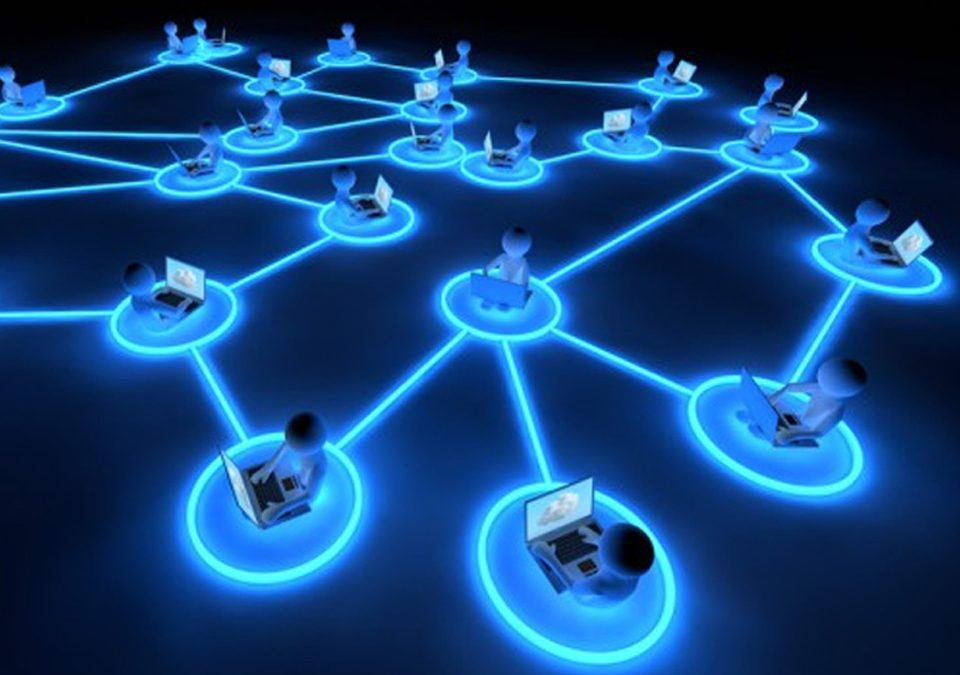
\includegraphics[width=0.6\textwidth]{img/programacao-orientada-objetos-fig.jpg}
	\caption{Ilustração de um sistema composto por partes (fonte: inputec).}
	\label{fig:programacao-orientada-objetos-fig}
\end{figure}

A ASOO permite a modelagem detalhada de cada uma dessas áreas, identificando os objetos, suas propriedades e comportamentos, além dos relacionamentos entre eles. Dessa forma, o software de gerenciamento de vendas da GeekStore será capaz de atender aos requisitos específicos de cada funcionalidade, proporcionando uma experiência eficiente e agradável tanto para a empresa quanto para os clientes.


\chapter{Processos de Negócio}\label{process_negocio} 

Os processos de negócio de todas as funções identificadas em Funções de Negócios\footnote{Funções de Negócios\textsuperscript{\ref{func_neg}}} foram devidamente identificados e numerados a seguir:

\begin{itemize}
    \item Controle de estoque:
    \begin{enumerate}
        \item Receber e conferir mercadorias
        \item Registrar entrada e saída de produtos
        \item Atualizar o saldo de estoque
        \item Realizar inventário regularmente
        \item Identificar e tratar produtos com prazo de validade expirado
        \item Gerenciar reposição de estoque
    \end{enumerate}
    
    \item Gerenciamento de vendas:
    \begin{enumerate}
        \item Registrar vendas realizadas
        \item Emitir notas fiscais ou recibos para os clientes
        \item Calcular o valor total das vendas
        \item Gerar relatórios de vendas por período, produto, cliente, etc.
        \item Realizar o fechamento de caixa
    \end{enumerate}
    
    \item Automação de vendas:
    \begin{enumerate}
        \item Implementar um sistema automatizado para registrar e processar vendas
        \item Permitir que os clientes façam pedidos online
        \item Integrar o sistema de vendas com o estoque e o sistema de gestão
    \end{enumerate}
    
    \item Módulos de acessibilidade:
    \begin{enumerate}
        \item Identificar as necessidades específicas de acessibilidade
        \item Implementar recursos e funcionalidades para tornar o sistema acessível
        \item Testar e validar a acessibilidade do sistema
        \item Realizar manutenção e atualizações regulares para garantir a continuidade da acessibilidade
    \end{enumerate}
    
    \item Gerenciamento de produtos raros:
    \begin{enumerate}
        \item Identificar os critérios para classificar um produto como raro
        \item Registrar e categorizar os produtos raros no sistema
        \item Monitorar o estoque e a disponibilidade dos produtos raros
        \item Implementar medidas especiais de segurança para proteger os produtos raros
    \end{enumerate}
    
    \item Cadastro de novos produtos:
    \begin{enumerate}
        \item Coletar informações detalhadas sobre os novos produtos
        \item Registrar as informações no sistema
        \item Atribuir categorias e características aos produtos
        \item Atualizar o estoque com os novos produtos
    \end{enumerate}
    
    \item Gerenciamento de promoções:
    \begin{enumerate}
        \item Planejar e definir as promoções a serem realizadas
        \item Definir os produtos participantes das promoções
        \item Calcular os descontos ou benefícios oferecidos nas promoções
        \item Divulgar as promoções para os clientes
        \item Monitorar o desempenho das promoções e avaliar os resultados
    \end{enumerate}
    
    \item Gerenciamento de pedidos:
    \begin{enumerate}
        \item Receber e processar pedidos dos clientes
        \item Verificar a disponibilidade dos produtos em estoque
        \item Confirmar os pedidos com os clientes
        \item Preparar os produtos para envio ou retirada
        \item Realizar o acompanhamento dos pedidos até a entrega final
        \item Solucionar possíveis problemas ou reclamações relacionados aos pedidos
    \end{enumerate}
\end{itemize}

\clearpage % Inicia uma nova página

\begin{figure}[htb] % Ambiente figure com a opção "p"
	\centering
	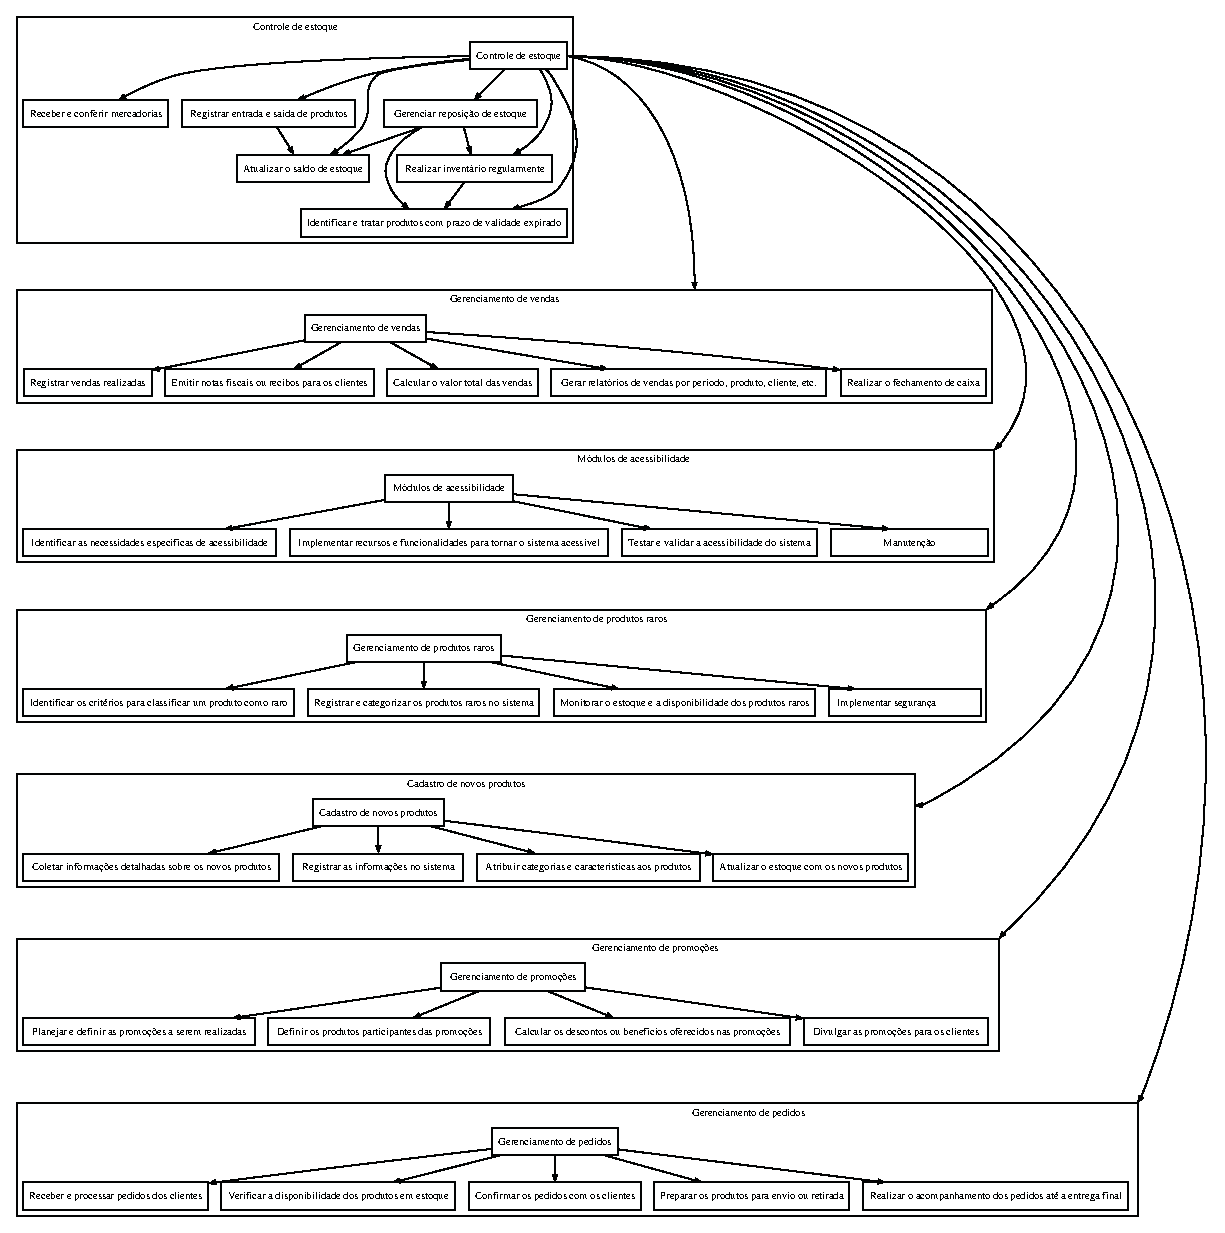
\includegraphics[width=\linewidth]{img/fluxograma.eps}
	\caption{Fluxograma representando os processos identificados (fonte:o autor)}
	\label{fig:fluxograma}
\end{figure}

\chapter{Automação de processos}\label{auto_process}

As automações de processos desempenham um papel fundamental na otimização e eficiência das operações de uma loja geek. Ao implementar essas automações, é possível agilizar tarefas rotineiras, reduzir erros humanos e melhorar a experiência tanto dos funcionários quanto dos clientes.

A primeira automação, a entrada de produtos, é realizada por meio da leitura de códigos de barras ou RFID. Essa tecnologia permite que o registro da entrada de produtos no estoque seja feito de forma rápida e precisa. Ao automatizar esse processo, as informações dos produtos são atualizadas automaticamente no sistema, evitando erros de digitação e agilizando a conferência. Isso resulta em uma gestão de estoque mais eficiente e precisa.

A automação do cálculo de estoque é alcançada por meio do uso de sensores de peso ou contadores automáticos. Esses sensores são integrados ao sistema de gestão, permitindo que o saldo de estoque seja atualizado de forma automática sempre que houver uma entrada ou saída de produtos. Com essa automação, a necessidade de contagens manuais frequentes é reduzida, proporcionando economia de tempo e minimizando erros de contagem.

A automação de pedidos online traz benefícios tanto para os clientes quanto para a loja. Ao implementar um sistema de pedidos online integrado ao estoque e ao sistema de vendas, os clientes têm a comodidade de fazer pedidos por meio de um site ou aplicativo. O sistema automatizado registra o pedido, verifica a disponibilidade dos produtos em estoque e envia uma confirmação para o cliente. Essa automação agiliza o processo de pedidos, reduzindo erros de comunicação e melhorando a satisfação do cliente.

A geração automática de relatórios de vendas é outra automação essencial. Configurando o sistema para gerar relatórios de vendas por período, produto, cliente, entre outros critérios, é possível obter insights sobre o desempenho das vendas de forma mais rápida e eficiente. Esses relatórios podem ser programados para serem gerados em intervalos regulares ou sob demanda, fornecendo informações valiosas para tomada de decisões estratégicas.

Por fim, a automação do acompanhamento de pedidos em tempo real proporciona uma experiência aprimorada tanto para os clientes quanto para a equipe de atendimento. Ao implementar um sistema de rastreamento de pedidos, é possível que os clientes acompanhem o status de seus pedidos desde o processamento até a entrega final. Isso reduz a necessidade de comunicação manual constante, oferece transparência e confiança aos clientes e melhora a eficiência da equipe de atendimento ao cliente.

\begin{quadro}[htb]
	\centering
	\caption{\label{quadro_automacao}Automações de processos}
	\resizebox{\textwidth}{!}{%
	\begin{tabular}{|p{1cm}|p{3.5cm}|p{8.5cm}|}
		\hline
		\textbf{Id} & \textbf{Função} & \textbf{Descrição} \\ \hline
		AP01 & Automação de entrada de produtos & Implementar um sistema de leitura de códigos de barras ou RFID para agilizar o registro da entrada de produtos no estoque. Isso permitiria que as informações dos produtos fossem automaticamente atualizadas no sistema, evitando erros de digitação e agilizando o processo de conferência. \\ \hline
		AP02 & Automação de cálculo de estoque & Utilizar sensores de peso ou contadores automáticos para monitorar o saldo de estoque. Os sensores podem ser integrados ao sistema de gestão, atualizando automaticamente o saldo de estoque sempre que uma entrada ou saída de produtos for registrada. Isso reduziria a necessidade de contagens manuais frequentes. \\ \hline
		AP03 & Automação de pedidos online & Implementar um sistema de pedidos online integrado ao estoque e ao sistema de vendas. Os clientes poderiam fazer pedidos através de um site ou aplicativo, e o sistema automatizado registraria o pedido, verificaria a disponibilidade dos produtos em estoque e enviaria uma confirmação para o cliente. Isso agilizaria o processo de pedidos e reduziria erros de comunicação. \\ \hline
		AP04 & Automação de geração de relatórios de vendas & Configurar o sistema para gerar automaticamente relatórios de vendas por período, produto, cliente, etc. Os relatórios poderiam ser programados para serem gerados em intervalos regulares ou sob demanda, fornecendo insights sobre o desempenho das vendas de forma mais rápida e eficiente. \\ \hline
		AP05 & Automação de acompanhamento de pedidos & Implementar um sistema de rastreamento de pedidos em tempo real, permitindo que os clientes e a equipe de atendimento ao cliente acompanhem o status dos pedidos desde o processamento até a entrega final. Isso reduziria a necessidade de comunicação manual constante e forneceria uma experiência melhor para os clientes. \\ \hline
	\end{tabular}%
	}
	\fonte{Autor.}
\end{quadro}

\chapter{Casos de Uso}\label{casos_de_usos}

A seguir, apresento os casos de uso correspondentes às operações que serão automatizadas na loja GeekStore:

\begin{enumerate}
    \item Caso de uso: Registro automático de entrada de produtos
    \begin{itemize}
        \item Ator: Funcionário responsável pelo controle de estoque
        \item Descrição: O funcionário utiliza o sistema para ler o código de barras ou RFID dos produtos recém-chegados, que são automaticamente registrados no estoque. As informações do produto são atualizadas no sistema, evitando erros de digitação e agilizando o processo de conferência.
    \end{itemize}
    
    \item Caso de uso: Cálculo automático de estoque
    \begin{itemize}
        \item Ator: Sistema de gestão de estoque
        \item Descrição: O sistema utiliza sensores de peso ou contadores automáticos para monitorar o saldo de estoque. Sempre que uma entrada ou saída de produtos é registrada, os sensores atualizam automaticamente o saldo de estoque. Isso reduz a necessidade de contagens manuais frequentes, tornando o processo mais eficiente.
    \end{itemize}
    
    \item Caso de uso: Pedidos online automatizados
    \begin{itemize}
        \item Ator: Cliente
        \item Descrição: Os clientes podem fazer pedidos de produtos através de um site ou aplicativo. O sistema automatizado registra o pedido, verifica a disponibilidade dos produtos em estoque e envia uma confirmação para o cliente. Esse processo agiliza a realização de pedidos e reduz erros de comunicação entre cliente e equipe de vendas.
    \end{itemize}
    
    \item Caso de uso: Geração automática de relatórios de vendas
    \begin{itemize}
        \item Ator: Sistema de gestão de vendas
        \item Descrição: O sistema é configurado para gerar automaticamente relatórios de vendas com base em critérios como período, produto, cliente, entre outros. Os relatórios podem ser programados para serem gerados em intervalos regulares ou sob demanda, fornecendo insights sobre o desempenho das vendas de forma rápida e eficiente.
    \end{itemize}
    
    \item Caso de uso: Acompanhamento automatizado de pedidos
    \begin{itemize}
        \item Ator: Cliente e equipe de atendimento ao cliente
        \item Descrição: O sistema implementa um sistema de rastreamento de pedidos em tempo real, permitindo que os clientes e a equipe de atendimento ao cliente acompanhem o status dos pedidos desde o processamento até a entrega final. Isso reduz a necessidade de comunicação manual constante e proporciona uma experiência melhor para os clientes.
    \end{itemize}
\end{enumerate}

Esses são os casos de uso correspondentes às automações de processos na loja geek. Cada caso de uso descreve uma interação específica entre o ator (usuário) e o sistema, detalhando o que o sistema faz em resposta às ações do usuário.

\chapter{Modelo de Casos de Uso}\label{modelo_de_casos_de_uso}

\section*{ Registro Automático de Entrada de Produtos}

\textbf{Descrição:} O funcionário responsável pelo controle de estoque utiliza o sistema para ler o código de barras ou RFID dos produtos recém-chegados, que são automaticamente registrados no estoque. As informações do produto são atualizadas no sistema, evitando erros de digitação e agilizando o processo de conferência.

\textbf{Fluxo Principal:}
\begin{enumerate}
  \item O funcionário seleciona a opção de registro de entrada de produtos no sistema.
  \item O sistema aguarda a leitura do código de barras ou RFID.
  \item O funcionário faz a leitura do código de barras ou RFID dos produtos.
  \item O sistema verifica a validade do código lido e busca as informações do produto associado.
  \item O sistema registra automaticamente a entrada dos produtos no estoque, atualizando as informações pertinentes.
  \item O sistema exibe uma confirmação de registro de entrada de produtos para o funcionário.
\end{enumerate}


\section*{ Cálculo Automático de Estoque}

\textbf{Descrição:} O sistema de gestão de estoque utiliza sensores de peso ou contadores automáticos para monitorar o saldo de estoque. Sempre que uma entrada ou saída de produtos é registrada, os sensores atualizam automaticamente o saldo de estoque. Isso reduz a necessidade de contagens manuais frequentes, tornando o processo mais eficiente.

\textbf{Fluxo Principal:}
\begin{enumerate}
  \item O sistema monitora continuamente os sensores de peso ou contadores automáticos.
  \item Quando uma entrada de produtos é registrada, o sensor atualiza o saldo de estoque, adicionando a quantidade de produtos ao saldo atual.
  \item Quando uma saída de produtos é registrada, o sensor atualiza o saldo de estoque, subtraindo a quantidade de produtos do saldo atual.
\end{enumerate}


\section*{ Pedidos Online Automatizados}

\textbf{Descrição:} Os clientes podem fazer pedidos de produtos através de um site ou aplicativo. O sistema automatizado registra o pedido, verifica a disponibilidade dos produtos em estoque e envia uma confirmação para o cliente. Esse processo agiliza a realização de pedidos e reduz erros de comunicação entre cliente e equipe de vendas.

\textbf{Fluxo Principal:}
\begin{enumerate}
  \item O cliente acessa o site ou aplicativo de pedidos online.
  \item O cliente navega pelos produtos disponíveis e seleciona os itens desejados.
  \item O sistema registra o pedido do cliente, armazenando as informações dos produtos selecionados.
  \item O sistema verifica a disponibilidade dos produtos em estoque.
  \item Se os produtos estiverem disponíveis, o sistema gera uma confirmação de pedido e envia ao cliente.
  \item Se algum produto estiver indisponível, o sistema informa ao cliente e fornece opções alternativas, se disponíveis.
  \item O cliente confirma o pedido e realiza o pagamento, se necessário.
\end{enumerate}


\section*{ Geração Automática de Relatórios de Vendas}

\textbf{Descrição:} O sistema é configurado para gerar automaticamente relatórios de vendas com base em critérios como período, produto, cliente, entre outros. Os relatórios podem ser programados para serem gerados em intervalos regulares ou sob demanda, fornecendo insights sobre o desempenho das vendas de forma rápida e eficiente.

\textbf{Fluxo Principal:}
\begin{enumerate}
  \item O usuário do sistema seleciona a opção de geração de relatórios de vendas.
  \item O usuário define os critérios do relatório, como período, produto, cliente, entre outros.
  \item O sistema busca os dados relevantes do banco de dados.
  \item O sistema gera o relatório com base nos dados selecionados.
  \item O sistema exibe o relatório para o usuário.
\end{enumerate}


\section*{ Acompanhamento Automatizado de Pedidos}

\textbf{Descrição:} O sistema implementa um sistema de rastreamento de pedidos em tempo real, permitindo que os clientes e a equipe de atendimento ao cliente acompanhem o status dos pedidos desde o processamento até a entrega final. Isso reduz a necessidade de comunicação manual constante e proporciona uma experiência melhor para os clientes.

\textbf{Fluxo Principal:}
\begin{enumerate}
  \item O cliente acessa o sistema de rastreamento de pedidos.
  \item O sistema solicita ao cliente o número do pedido ou informações de identificação.
  \item O sistema busca as informações do pedido no banco de dados.
  \item O sistema exibe o status atual do pedido, como processamento, embalagem, transporte, etc.
  \item O cliente pode acompanhar o progresso do pedido em tempo real.
\end{enumerate}

\chapter{Relacionamentos e Requisitos Não Funcionais}\label{rel_e_requi_NF}

\section{Relacionamentos entre casos de uso}\label{rel_entre_casos}

\begin{enumerate}
	\item O caso de uso "Registro Automático de Entrada de Produtos" pode incluir o caso de uso "Cálculo Automático de Estoque", pois a entrada de produtos afeta o cálculo do saldo de estoque.
	\item O caso de uso "Pedidos Online Automatizados" pode incluir o caso de uso "Registro Automático de Entrada de Produtos", uma vez que o registro de entrada de produtos ocorre quando um pedido é feito e produtos são adicionados ao estoque.
	\item O caso de uso "Pedidos Online Automatizados" também pode incluir o caso de uso "Acompanhamento Automatizado de Pedidos", pois, após fazer um pedido, os clientes podem acompanhar o status do pedido através do sistema de rastreamento.
	\item O caso de uso "Geração Automática de Relatórios de Vendas" não apresenta relacionamentos diretos com outros casos de uso neste conjunto.
\end{enumerate}

\section{Requisitos Não Funcionais }\label{req_n_func}

\begin{itemize}
	\item Desempenho: O sistema deve ser capaz de lidar com um grande volume de transações, processando-as de forma eficiente e mantendo tempos de resposta rápidos.
	\item Segurança: O sistema deve garantir a proteção dos dados dos clientes, produtos e transações, implementando medidas de segurança, como criptografia e autenticação adequadas.
	\item Usabilidade: O sistema deve ser intuitivo e fácil de usar, tanto para os funcionários responsáveis pelo controle de estoque quanto para os clientes que acessam o site ou aplicativo de pedidos online. Deve ser fornecida uma interface amigável e instruções claras para facilitar a interação com o sistema.
	\item Confiabilidade: O sistema deve ser altamente confiável, garantindo que as transações sejam registradas corretamente, que os dados estejam sempre disponíveis e que não ocorram perdas de informações importantes.
	\item Escalabilidade: O sistema deve ser capaz de lidar com o crescimento do volume de dados e transações ao longo do tempo, sem comprometer seu desempenho e funcionalidade.
	\item Manutenibilidade: O sistema deve ser desenvolvido de forma modular e organizada, facilitando a manutenção, atualização e expansão futuras.
	\item Integração: O sistema deve ser capaz de se integrar a outros sistemas existentes na empresa, como bancos de dados, sistemas de pagamento e sistemas de logística, garantindo a troca de informações de forma eficiente e precisa.
\end{itemize}

\chapter{Contexto de Uso}\label{contex_de_uso}

O contexto de uso do sistema envolve usuários, tarefas e ambiente em que o sistema será utilizado. Com base nos casos de uso identificados, podemos identificar o seguinte contexto de uso:

\section{Usuários}\label{usuarios_contex_uso}

\begin{enumerate}
	\item Funcionário responsável pelo controle de estoque: Este usuário utiliza o sistema para registrar a entrada de produtos, ler códigos de barras ou RFID, verificar informações de produtos e conferir o estoque.
	\item Clientes: Os clientes utilizam o site ou aplicativo para fazer pedidos de produtos, navegar pelos itens disponíveis, acompanhar o status dos pedidos e realizar pagamentos, quando necessário.
	\item Usuário do sistema (administrador): Este usuário é responsável por configurar o sistema, definir critérios para a geração de relatórios de vendas e acessar os relatórios gerados.
\end{enumerate}

\section{Tarefas executadas pelos usuários}\label{Tarefas_usuarios_contex_uso}

\begin{enumerate}

	\item Funcionário responsável pelo controle de estoque:

	\begin{itemize}
		\item Selecionar a opção de registro de entrada de produtos no sistema.
		\item Realizar a leitura dos códigos de barras ou RFID dos produtos.
		\item Verificar a validade dos códigos lidos e buscar informações dos produtos associados.
		\item Registrar a entrada dos produtos no estoque.
		\item Conferir as informações pertinentes e visualizar a confirmação de registro de entrada de produtos.
	\end{itemize}

	\item 	Clientes:

	\begin{itemize}
		\item Acessar o site ou aplicativo de pedidos online.
		\item Navegar pelos produtos disponíveis e selecionar os itens desejados.
		\item Registrar o pedido e fornecer as informações necessárias.
		\item Verificar a disponibilidade dos produtos em estoque.
		\item Receber a confirmação do pedido e, se necessário, fornecer informações de pagamento.
		\item Acompanhar o status do pedido em tempo real.
	\end{itemize}

	\item 	Usuário do sistema (administrador):

	\begin{itemize}
		\item Selecionar a opção de geração de relatórios de vendas.
		\item Definir critérios do relatório, como período, produto, cliente, entre outros.
		\item Buscar os dados relevantes do banco de dados.
		\item Gerar o relatório com base nos critérios definidos.
		\item Visualizar o relatório gerado.
	\end{itemize}

\end{enumerate}


\section{Ambiente de uso}\label{ambientes_de_uso}

O sistema é utilizado em um ambiente empresarial, onde as tarefas de controle de estoque, registro de entrada e saída de produtos, gerenciamento de pedidos e geração de relatórios de vendas são realizadas. O sistema pode ser acessado por meio de um computador ou dispositivos móveis, como smartphones ou tablets, tanto pelos funcionários responsáveis pelo controle de estoque quanto pelos clientes que desejam fazer pedidos online. O ambiente deve ser conectado à internet para permitir a comunicação entre o sistema e os dispositivos dos usuários, bem como o acesso aos dados armazenados no banco de dados do sistema.

\chapter{Regras de Negócio e Glossário}\label{regras_de_negocio_e_glossario}

\section{Regras de Negócio}\label{regras_de_negocio}

\begin{quadro}[htb]
	\centering
	\caption{\label{quadro_regras_negocio}Regras de Negócio}
	\resizebox{\textwidth}{!}{%
	\begin{tabular}{|p{1cm}|p{3.5cm}|p{8.5cm}|}
		\hline
		\textbf{Id} & \textbf{Regra de Negócio} & \textbf{Descrição} \\ \hline
		RG-N01 & Produtos com estoque abaixo de um determinado limite não podem ser vendidos & O sistema deve verificar o saldo de estoque de um produto antes de permitir que ele seja incluído em um pedido. Se o estoque estiver abaixo de um limite predefinido, o sistema deve informar ao cliente que o produto não está disponível para venda. \\ \hline
		RG-N02 & A validade do código de barras ou RFID lido deve ser verificada & O sistema deve validar o código de barras ou RFID lido pelo funcionário responsável pelo controle de estoque. Caso o código não seja válido, o sistema deve exibir uma mensagem de erro e solicitar uma nova leitura. \\ \hline
		RG-N03 & O sistema deve buscar as informações do produto associadas ao código lido & Após a leitura do código de barras ou RFID, o sistema deve buscar as informações relevantes do produto no banco de dados, como nome, descrição, preço, etc., para atualizar o registro de entrada de produtos e exibir as informações pertinentes. \\ \hline
		RG-N04 & O sistema deve calcular e atualizar o saldo de estoque automaticamente & Após a leitura do código de barras ou RFID e a confirmação da validade do código, o sistema deve registrar automaticamente a entrada do produto no estoque, adicionando a quantidade correspondente ao saldo atual. Da mesma forma, quando uma saída de produtos é registrada, o sistema deve subtrair a quantidade de produtos do saldo atual. \\ \hline
		RG-N05 & O sistema deve fornecer opções alternativas se algum produto estiver indisponível & Se algum produto selecionado pelo cliente não estiver disponível em estoque, o sistema deve informar ao cliente sobre a indisponibilidade e sugerir opções alternativas, se houver, com base nas características dos produtos desejados. \\ \hline
	\end{tabular}%
	}
	\fonte{Autor.}
\end{quadro}

\section{Glossário}\label{glossario}

\begin{table}[htb]
	\centering
	\caption{\label{tab:glossario}Glossário de Termos e Conceitos I}
	\begin{tabular}{|p{3.5cm}|p{10cm}|}
		\hline
		\textbf{Termo} & \textbf{Descrição} \\
			\hline
			Código de barras & Um código visual composto por barras e espaços que representa informações sobre um produto, permitindo sua identificação única. \\
			\hline
			RFID (Radio-Frequency Identification) & Uma tecnologia de identificação por radiofrequência que utiliza tags eletrônicas para armazenar e recuperar dados remotamente. No contexto do sistema, as tags RFID são utilizadas para identificar produtos. \\
			\hline
			Estoque & O conjunto de produtos ou itens mantidos por uma empresa para venda ou uso posterior. O estoque representa a quantidade disponível de cada produto em um determinado momento. \\
			\hline
			Sistema de gestão de estoque & Um sistema utilizado para controlar e monitorar o estoque de uma empresa, incluindo atividades como registro de entrada e saída de produtos, atualização de saldo de estoque e geração de relatórios. \\
			\hline
			Pedido & Uma solicitação feita por um cliente para adquirir um ou mais produtos específicos. O pedido geralmente inclui informações sobre os produtos selecionados, quantidade desejada e informações de entrega. \\
			\hline
			Banco de dados & Um sistema organizado de armazenamento de dados que permite a recuperação, manipulação e análise eficiente das informações. No contexto do sistema, o banco de dados é utilizado para armazenar informações sobre produtos, clientes, pedidos e outras entidades relacionadas. \\
			\hline
			Usuário & Uma pessoa que interage com o sistema, executando tarefas e utilizando suas funcionalidades. Os usuários podem incluir funcionários responsáveis pelo controle de estoque, clientes e administradores do sistema. \\
			\hline
			Funcionário responsável pelo controle de estoque & Um membro da equipe de uma empresa que é responsável por monitorar e registrar a entrada e saída de produtos, manter o estoque atualizado e realizar tarefas relacionadas ao controle de estoque. \\
			\hline
	\end{tabular}
	\fonte{Autor.}
\end{table}

\begin{table}[htb]
	\centering
	\caption{\label{tab:glossarioII}Glossário de Termos e Conceitos II}
	\begin{tabular}{|p{3.5cm}|p{10cm}|}
		\hline
		\textbf{Termo} & \textbf{Descrição} \\
			\hline
			Cliente & Uma pessoa ou organização que faz pedidos de produtos através do site ou aplicativo do sistema. Os clientes podem navegar pelos produtos, selecionar itens, fazer pedidos e acompanhar o status de seus pedidos. \\
			\hline
			Relatório de vendas & Um documento que apresenta informações sobre as vendas de produtos em um determinado período de tempo. Os relatórios de vendas fornecem insights sobre o desempenho das vendas, incluindo dados como quantidade vendida, receita gerada, produtos mais vendidos, entre outros. \\
			\hline
			Sistema automatizado & Um sistema que realiza tarefas de forma automática, sem intervenção humana direta. No contexto do sistema, são utilizadas automações para registrar a entrada de produtos, atualizar o saldo de estoque, gerar confirmações de pedidos, entre outras funcionalidades. \\
			\hline
			Disponibilidade & A condição de um produto estar em estoque e disponível para venda. A disponibilidade é verificada pelo sistema antes de confirmar um pedido, garantindo que o produto esteja disponível em quantidade suficiente. \\
			\hline
	\end{tabular}
	\fonte{Autor.}
\end{table}

\part{Banco de Dados}

\chapter{Diagrama de Classes de Análise}\label{diagrama_de_classes_def}

O diagrama de classes de análise é uma representação visual das principais classes e suas interações em um sistema, focando na análise dos requisitos e na estrutura do domínio do problema. Ele é usado para identificar as entidades (classes), interfaces (fronteiras) e controladores (lógica de negócio) do sistema, ajudando a entender como as diferentes partes do sistema se relacionam e interagem entre si.

O objetivo do diagrama de classes de análise é capturar as principais classes conceituais do sistema, seus atributos e relacionamentos, sem se preocupar com detalhes de implementação. Ele fornece uma visão geral das classes envolvidas no sistema e como elas se relacionam, permitindo uma análise mais aprofundada das funcionalidades e requisitos do sistema.

Ao criar um diagrama de classes de análise, é comum identificar as principais entidades do domínio do problema e suas características relevantes, bem como as interfaces através das quais o sistema interage com usuários externos ou outros sistemas. Os controladores representam a lógica de negócio do sistema, responsável por coordenar as operações e manipular os dados entre as entidades e as interfaces.

Em resumo, o diagrama de classes de análise é uma ferramenta de modelagem que ajuda a visualizar a estrutura conceitual do sistema, permitindo uma compreensão mais clara dos elementos envolvidos e suas relações, auxiliando na análise e no planejamento do sistema antes da implementação.

\clearpage

\section{Diagrama de Classes e Dados}\label{diagrama_de_classes}

\begin{figure}[htb] % Ambiente figure com a opção "p"
	\centering
	\includegraphics[width=\linewidth]{img/diagrama-de-classes.eps}
	\caption{Diagrama de classes do projeto (fonte:o autor)} 
	\label{fig:diagrama_de_classes}
\end{figure}

%\footnote{\url{https://www.pimvi.orbytesistemas.com/redirect}}

%redireciona para https://mermaid.live/edit#pako:eNrdV0tu2zAQvQrBlZzaQeRfHC0KBElaZFEgaIEuWnVBU4xLVCIdkTKaBDlNFzlA0RP4YqVI_ShRttNFFl2ZGr4h570ZkuNHiHlEYABxjIS4pGiVoiRkAOhvcCUkv8sIeMxNAIwAlYSJAFxLknz9ZoxvAIooppyhNDd7CpIYxCAAG06jEpaShG_IHhCSGYrpw761lpnABQZvf0d0xQMgZErZamDwJTCmQmogE96gGfhTyGqenwmLkKhpbvR3YOw10ZSY2LTZ06AC0woPI4ZJfADQ8DCwLhFtt5mYSL2BFZvF5TyTPEEY8f-EDiZC0CWNaYSiRiUiyx6AJecxQayuI7pBqe3staKNiDgEpmqW3lLsgjU2tYK-SXmk0iA-opQ3ymrdNAclKv9yHKbGrFc4Wi7u0_VCr-q4vdDPJLrp1E13Y9ZOuqWON3AIYYl5gVSJyJR3daw8--XrkNkp2z50W659eEumfonc8jSUcajynqSEYYoSwqQtTcIxJ0YbNUQNcXBK9fLa7K2LQY3s1eZAh6Y8B7pUChm8UyI91dHI0PQGbaL9Kt2QiEbWeTQGtYIetIXSRs-ASkzPzXgItqBqkA6ieqJF0wToDewQLYr5k1ZTaq1bmhlPSNt2lyEmi9uTZcmSpHURke0zb1lHgJhuICjbAvczujeWCEn1fFwiSXZ0FSMguURxJwYcU5VKFcOFGfRdvfld8k-qOLk3tLoqRbABlN3yNEHb5-0fIs6LS4iK1urF-TSonYVb0HhFCu786gln_9Ag84vb57TNRE_8ExX1RGPOZIdMXkPXLFfZrqTc_o4mlrH3vbDD1Ofr9Yv34AALnzpCl14kQTTuFF1v_lz3X7Fp2fqPRm9BCP0QmosmAHk-EGUiBxV9s8EcKYy5AQJ1HHCcqeTloLohzXHGRdvtzi6frKD5vN1E1Xs0T7i9U9UpdMAtoP14WmhTqzvg5SvS8DKlY_uUGxvtlNhmUMqqekcSc7YSwDz_RrgWuEx5H_ioCXYzrRgdhjZMDgyjQlcruxWHQ5gQdTnSSP3R1OUbQvmdJCSEgRpGKP0RwpA9KRxSnp_uGYbBLYoFGcJsrU4cKf6YVtY1Yl84V98yzcwnDB7hTxhM_GN_OllMpyf-eD6dTxanQ3gPg9FkdnI8Hk9OF_PJdHo2PfOfhvBBr-AfLyaz8dnJYjzz_fl85g-hoiV5-qH4Y5z_PP0FCSwMzQ

\clearpage

\section{Classes}

\begin{itemize}
    \item \texttt{Acessibilidade}: representa os módulos de acessibilidade do sistema. Possui métodos para ativar, desativar e verificar a acessibilidade do sistema, permitindo que usuários com necessidades específicas possam utilizar o sistema de forma adequada.
    
    \item \texttt{Automação}: responsável pela automação das vendas. Herda os métodos da classe \texttt{Vendas} e permite realizar e cancelar vendas. Essa classe é utilizada para automatizar o processo de vendas, facilitando a interação com o sistema.
    
    \item \texttt{Cadastro}: responsável pelo cadastro de novos produtos. Possui métodos para adicionar, remover e atualizar produtos, bem como buscar produtos por código e listar todos os produtos cadastrados.
    
    \item \texttt{Cliente}: representa um cliente do sistema. Possui atributos como nome e email, e está associado a vendas e pedidos.
    
    \item \texttt{Estoque}: representa o estoque de produtos da empresa. Possui métodos para adicionar, remover e atualizar itens no estoque, bem como buscar itens por código e listar todos os itens presentes no estoque.
    
    \item \texttt{Gerenciamento}: responsável pelo gerenciamento de promoções. Possui métodos para criar, remover e atualizar promoções, bem como buscar promoções por código e listar todas as promoções disponíveis.
    
    \item \texttt{GerenciamentoPedidos}: responsável pelo gerenciamento de pedidos. Possui métodos para criar, cancelar, buscar e listar pedidos realizados.
    
    \item \texttt{Item}: representa um item de estoque ou venda. Possui atributos como código, nome, quantidade e preço, e é utilizado tanto pelo estoque quanto pelas vendas.
    
    \item \texttt{Pedido}: representa um pedido realizado. Possui atributos como código, data, itens e total, e está associado a um cliente e a um ou mais produtos.
    
    \item \texttt{Produto}: representa um produto comum. Possui atributos como código, nome, preço, quantidade em estoque e está associado ao estoque e às vendas. Além disso, pode ser relacionado a uma promoção específica.
    
    \item \texttt{ProdutoRaro}: representa um produto raro. Possui atributos como código, nome, preço, quantidade em estoque e informações adicionais. Além disso, está associado a promoções específicas.
    
    \item \texttt{Promocao}: representa uma promoção. Possui atributos como código, nome, desconto, data de início e data de fim, e está associada a um ou mais produtos.
    
    \item \texttt{Vendas}: é responsável pelo gerenciamento das vendas realizadas. Possui métodos para realizar vendas, cancelar vendas, buscar vendas por código e listar todas as vendas efetuadas.
    
    \item \texttt{Venda}: representa uma venda realizada. Possui atributos como código, data, itens e total, e está associada a um cliente.
\end{itemize}


% ----------------------------------------------------------
% Finaliza a parte no bookmark do PDF
% para que se inicie o bookmark na raiz
% e adiciona espaço de parte no Sumário
% ----------------------------------------------------------
\phantompart

% ---
% Conclusão
% ---
\chapter{Conclusão}
% ---


\chapter{Conclusão}

Neste trabalho, foi realizado um estudo aprofundado sobre os requisitos e necessidades de uma loja específica de jogos, acessórios e produtos geek, visando o desenvolvimento de um sistema de controle de vendas personalizado. O objetivo principal foi substituir o uso de planilhas em Excel por uma solução mais eficiente e automatizada, proporcionando uma gestão mais eficaz das vendas e um atendimento personalizado aos clientes.

Durante o desenvolvimento do sistema, foram aplicados conceitos de Análise de Sistemas Orientada a Objetos, Banco de Dados e Gestão Estratégica de Recursos Humanos. Essas disciplinas foram fundamentais para o planejamento, modelagem e implementação do sistema, garantindo a integridade dos dados, a otimização dos processos e a consideração da acessibilidade para usuários com deficiência.

O sistema desenvolvido apresenta funcionalidades abrangentes, incluindo o controle de estoque, gerenciamento de vendas e consideração da raridade e disponibilidade dos produtos. Com a automatização desses processos, espera-se que a loja obtenha melhorias significativas em sua eficiência operacional, reduzindo erros e retrabalho, além de proporcionar uma melhor experiência para os clientes.

Durante o desenvolvimento do projeto, enfrentamos desafios e tomamos decisões importantes para alcançar os objetivos propostos. A colaboração e o trabalho em equipe foram fundamentais para o sucesso do projeto, permitindo a troca de ideias, a identificação de problemas e a busca por soluções eficazes.

A partir deste estudo, é possível afirmar que a implementação do sistema de controle de vendas personalizado trará benefícios significativos para a loja em termos de gestão e atendimento ao cliente. Recomenda-se a realização de testes adicionais e a realização de um treinamento adequado para os funcionários, a fim de garantir uma transição suave para o novo sistema e maximizar seus benefícios.

Por fim, espera-se que este projeto possa servir como base para futuras melhorias e expansões do sistema, atendendo às necessidades em constante evolução da loja e contribuindo para o seu crescimento no mercado.

\vspace{\baselineskip}

\noindent
\textbf{Palavras-chave:} análise de requisitos. sistema de controle de vendas. loja geek. software desktop. acessibilidade. estoque. gerenciamento de vendas.

% ----------------------------------------------------------
% ELEMENTOS PÓS-TEXTUAIS
% ----------------------------------------------------------
\postextual
% ----------------------------------------------------------

% ----------------------------------------------------------
% Referências bibliográficas
% ----------------------------------------------------------
\bibliography{abntex2-modelo-references}

\begin{itemize}
    \item Alura. (s.d.). POO: Programação Orientada a Objetos, 2023 \\
	Disponível em: \url{https://www.alura.com.br/artigos/poo-programacao-orientada-aobjetos}
    \item FERREIRA, J. (s.d.). Aula 4 - Interfaces. Disponível em:\\
	\url{https://sites.google.com/site/anhangueraniteroipoo/aulas/aula-4---interfaces}
    \item CODIFICAR. (s.d.). Requisitos Funcionais e Não Funcionais: o que são e como
	identificá-los. Dísponivel em:\\ \url{https://codificar.com.br/requisitos-funcionais-naofuncionais/}
	\item DEV MEDIA. Revista Engenharia de Software
	\url{https://www.devmedia.com.br/introducaoa-engenharia-de-requisitos/8034}
	\item REDEQUISITOS. Quais os tipos de Requisitos de Software? Sabe a diferença
	entre eles?. Disponível em:\\
	\url{http://rederequisitos.com.br/quais-os-tipos-derequisitos-desoftware-sabe-diferenca-entre-eles/}
	\item REQUISITOS DE SISTEMA:\url{https://codificar.com.br/requisitos-funcionais-naofuncionais/#:~:text=Os%20requisitos%20funcionais%20descrevem%20o,qu}
	
\end{itemize}

%---------------------------------------------------------------------
% INDICE REMISSIVO
%---------------------------------------------------------------------
\phantompart
\printindex
%---------------------------------------------------------------------

\end{document}
